\begin{problem}{Pýramídi}{Inn}{Út}{~}{~}

	\begin{wrapfigure}{r}{0.35\textwidth}
		\vspace{-25pt}
		\begin{center}
			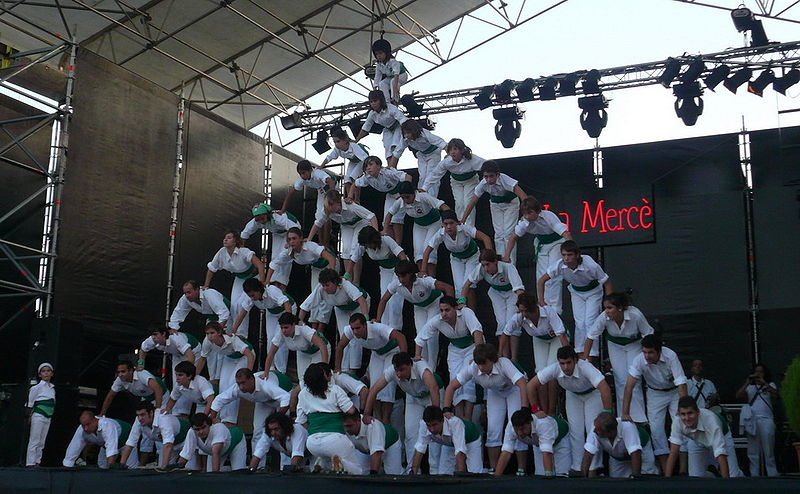
\includegraphics[scale=0.2]{../Pyramidi/pyramid.jpg}
		\end{center}
		\vspace{-30pt}
	\end{wrapfigure}

	Eftir skemmtilega forritunarkeppni ætla keppendurnir að fara út og klára daginn með stæl.
	Þeir ákveða að búa til mannlegan pýramída þar sem einn keppandi er á toppnum, tveir eru fyrir neðan hann, þrír eru fyrir neðan þá og svo framvegis.
	Ekki er samt víst að allir komist í pýramídann. Til dæmis gætu þeir gert þrjár hæðir, en ekki haft nóg af fólki til að gera fjórðu hæðina.
	Lestu inn fjölda keppenda og skrifaðu út hæð hæsta pýramídans sem þeir geta búið til og hversu margir yrðu þá útundan.

	\Input

		Á fyrstu línu er heiltalan $1 \leq T \leq 100$, sem táknar fjölda prófunartilvika sem fylgja. Hvert prófunartilvik samanstendur af einni línu með heiltölunni $1 \leq N \leq 10^7$, þar sem $N$ táknar fjölda keppenda.

	\Output

		Fyrir hvert prófunartilvik á að skrifa út eina línu sem inniheldur tvær heiltölur, aðskildar með bili. Fyrri heiltalan táknar hæsta pýramída sem hægt er að búa til, en seinni heiltalan táknar fjölda keppenda sem verða þá útundan.

	\Examples


\begin{example}
\exmp{%
4
31
10
2
1234572
}{%
7 3
4 0
1 1
1570 1337
}%
\end{example}
\end{problem}